\section{Appendix}
\label{appendix:scenarios}


This appendix presents the scenarios that were presented to the participants of the study and the raw data
summarizing each group's discussion and findings. The scenarios were presented to the participants to evaluate
the types of competitive advantages that could arise from using adaptive hybrid intelligence in the context
of the described scenario. The participants were first introduced to adaptive hybrid intelligence
and competitive advantages for enterprises from using AI. Then, they were asked to discuss the
following scenarios in groups of 6-8 participants and to record their thoughts and findings.


\subsection{Scenario 1: Writing Manuscripts}

\subsubsection*{Scenario}

Web-based platforms for authors to write their manuscript is typically not part of the offering of
publishers. Let's now assume that a publisher would launch a tooling that allows authors to write
their papers on the publisher's platform. The publisher could support authors by deploying adaptive
AI tools---similar to GitHub Copilot for coding---to write the scientific manuscript. How and why
should the tool be a hybrid AI that adapts to the author? How can it adapt to the author? How would
such a system bring a competitive advantage to publishers?

\subsubsection*{Results}

The results for this scenario are shown in Figure~\ref{fig:appendix:fig1}.

\begin{figure}[h!]
    \centering
    \caption{Scenario 1: Writing Manuscripts}
    \label{fig:appendix:fig1}
    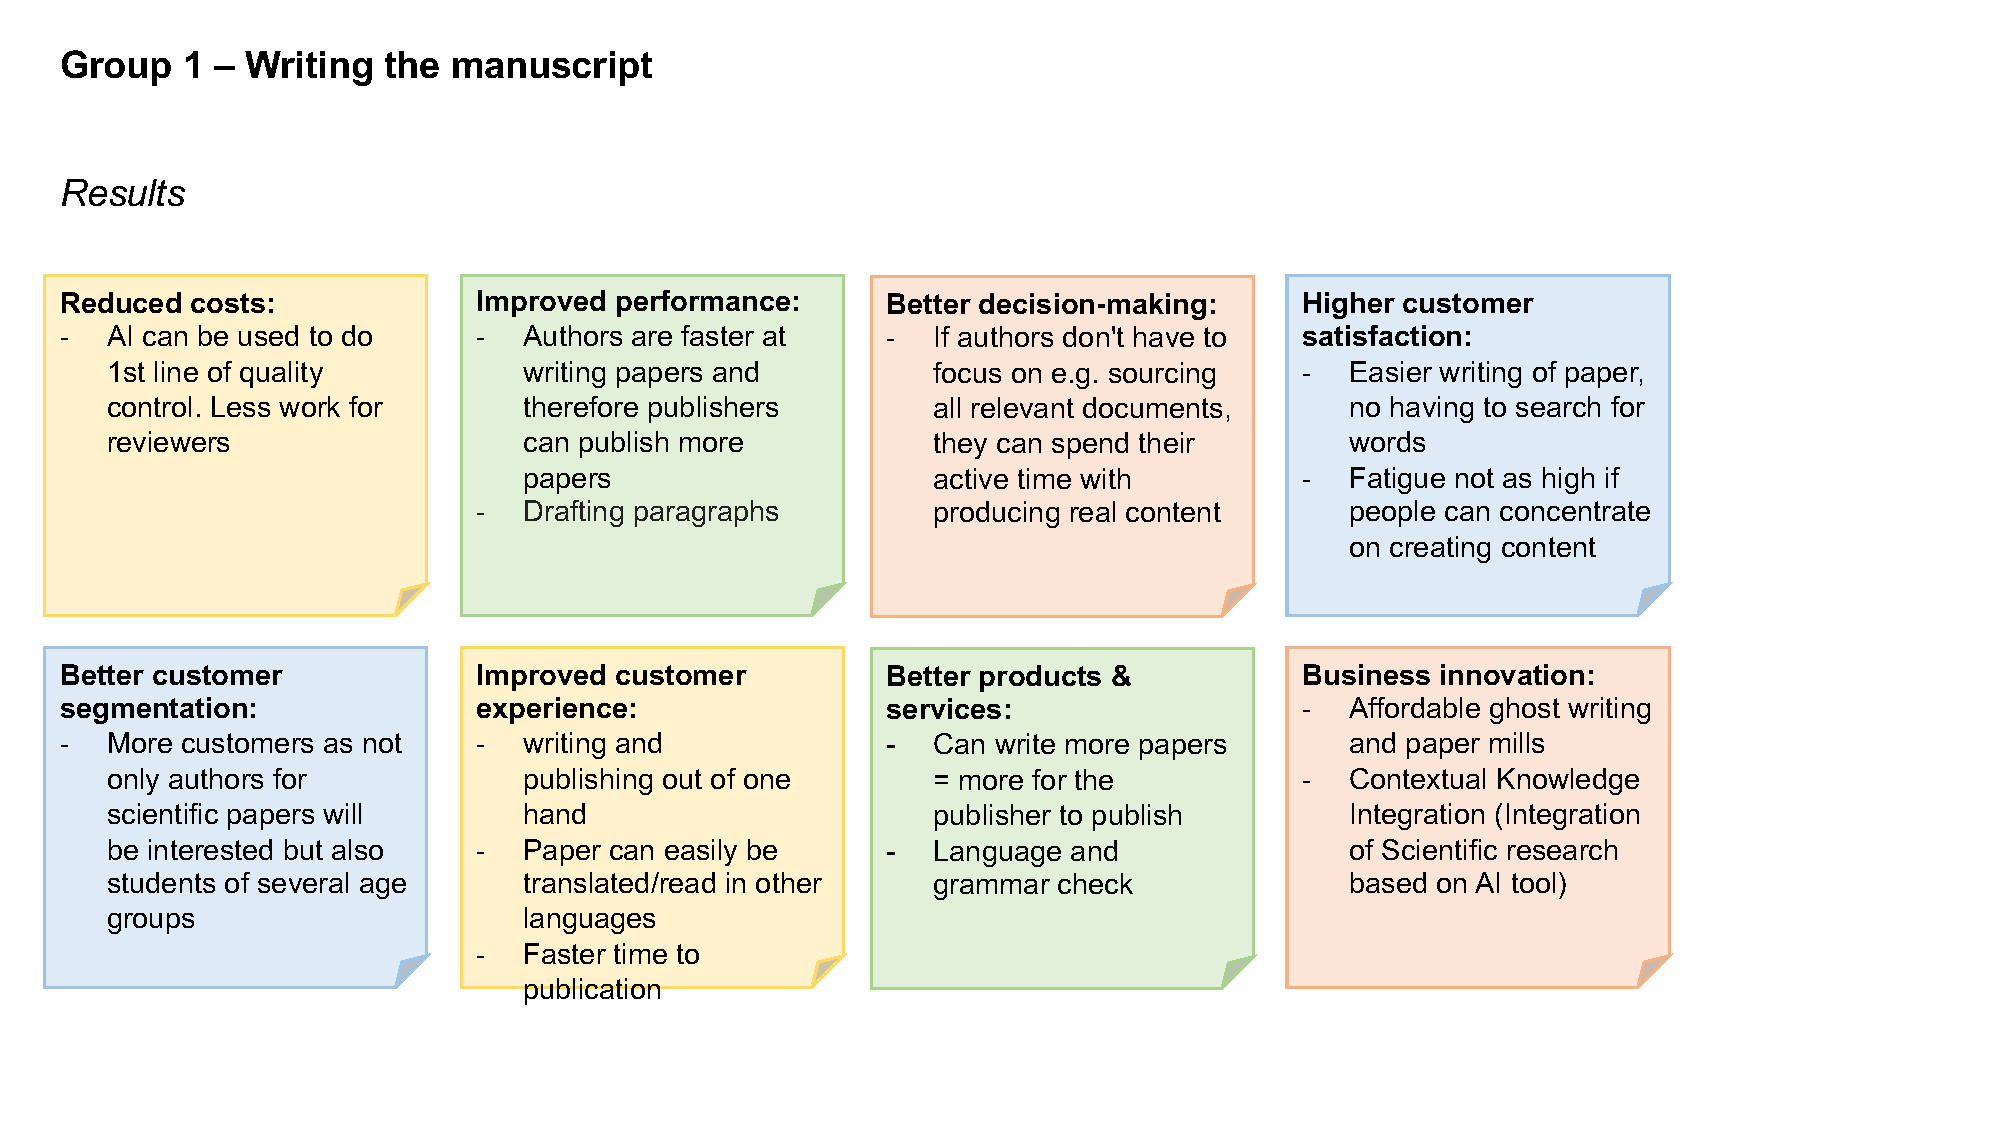
\includegraphics[width=\textwidth]{figures/results_1.pdf}
\end{figure}


\newpage
\subsection{Scenario 2: Finding Journals \& Formatting Manuscripts}

\subsubsection*{Scenario}

There are 1000s of journals---alone 260 journals contain “information systems” in the title. Imagine
you are an author and just finished writing your manuscript. You are now looking at options where you
could publish your manuscript. How and why could an adaptive, hybrid AI system support you as the author
in recommending suitable journals---considering that you may have specific wishes (maybe a journal in
information system that accept more technical contributions, or with authors predominantly from the D-A-CH
region, or a journal published in German). As an author you will typically also be asked to comply with the
style of the journal that you chose. How can it adapt to or learn from the author (e.g., history of previous
recommendations)? How would such a system bring a competitive advantage to publishers? Think of reformatting
the manuscript, if the author was rejected in another journal and now resubmits to your journal.

\subsubsection*{Results}

The results for this scenario are shown in Figure~\ref{fig:appendix:fig2}.

\begin{figure}[h!]
    \centering
    \caption{Scenario 2: Finding Journals \& Formatting Manuscripts}
    \label{fig:appendix:fig2}
    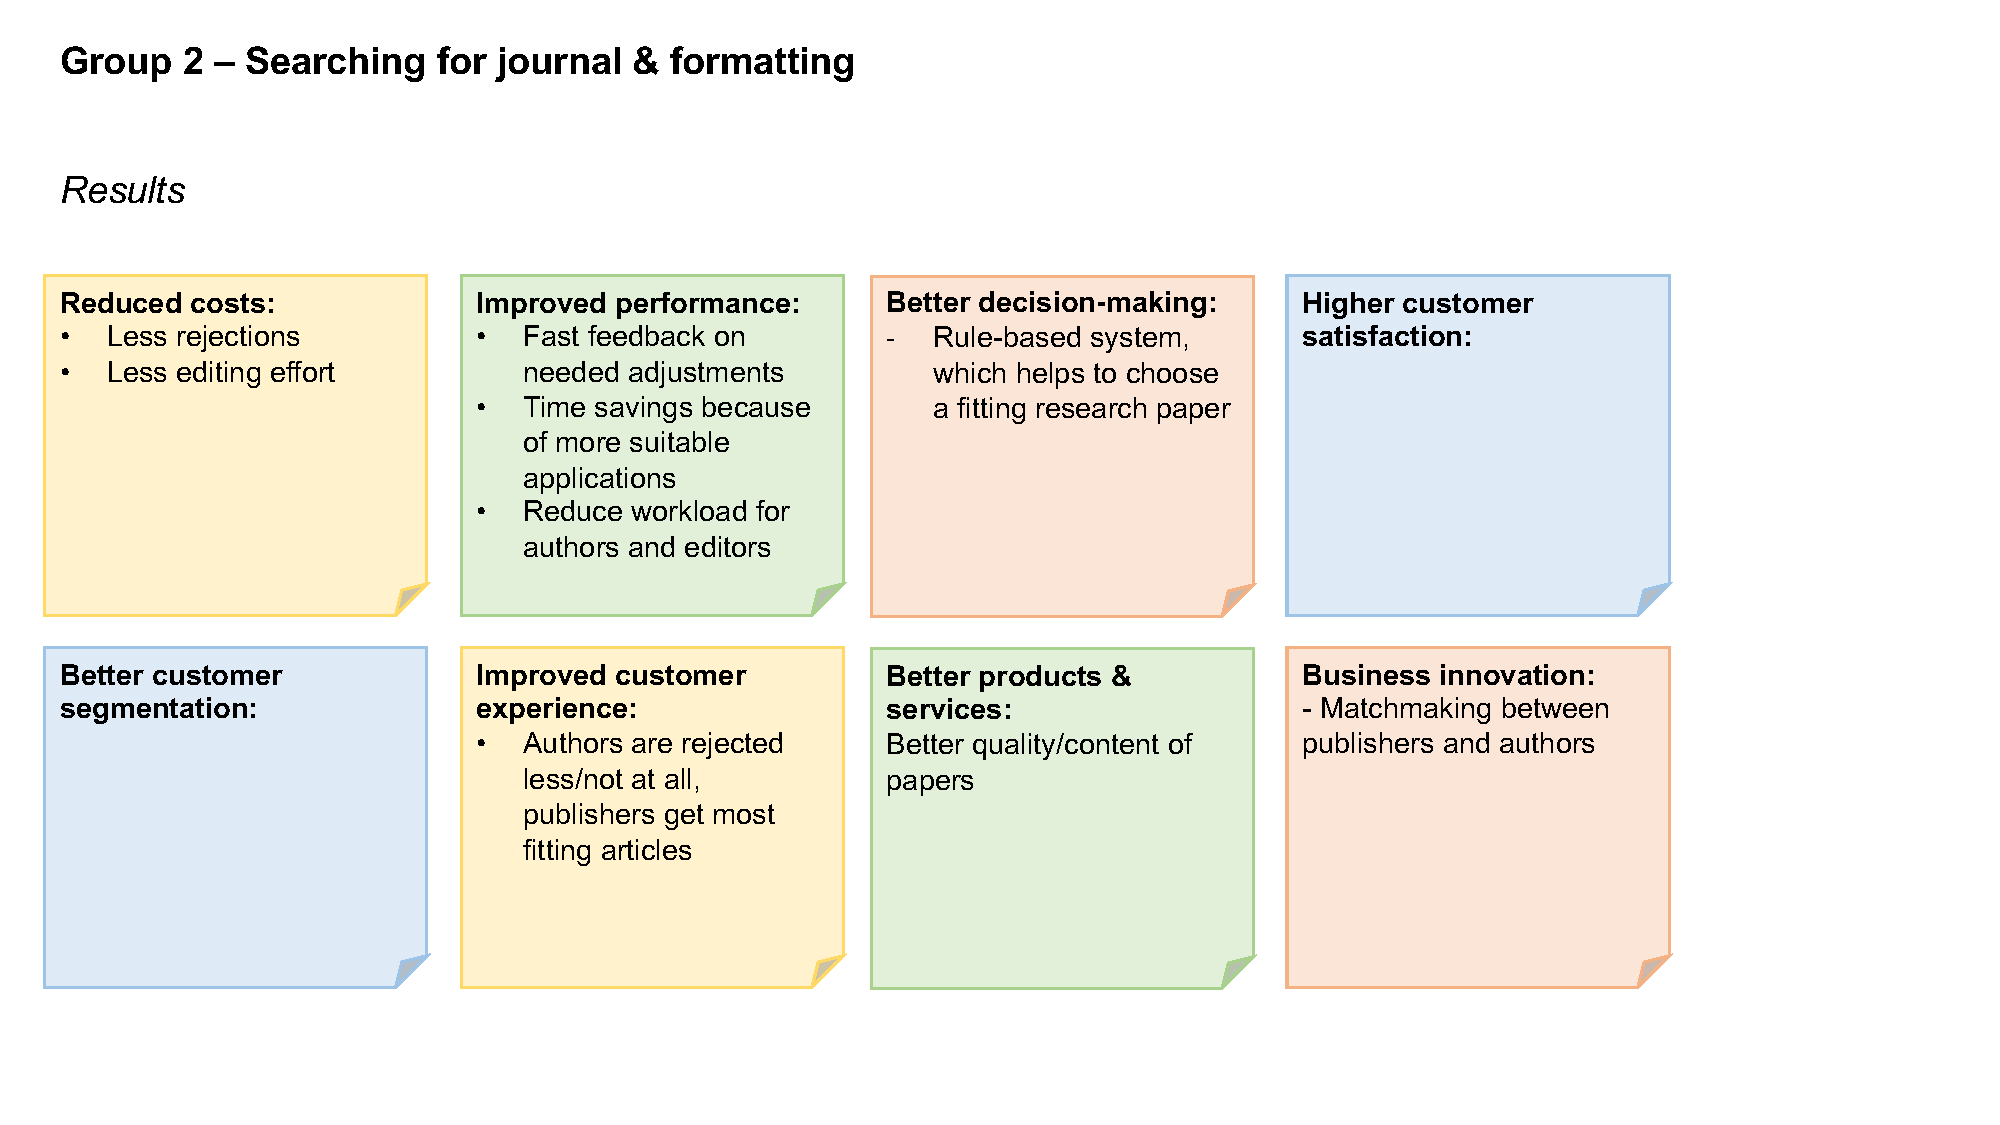
\includegraphics[width=\textwidth]{figures/results_2.pdf}
\end{figure}


\newpage
\subsection{Scenario 3: Desk Review of Manuscripts}

\subsubsection*{Scenario}

As part of desk review, editors are confronted with an increasing number of ethical problems. This could be
completely fake (AI generated) papers, authorship issues (adding authors that did not contribute to the manuscript),
fabricated images and data, citation to references that are irrelevant to the work, etc. Doing these checks manually
is laborious. Yet, automating with narrow AI is difficult as there are only few data examples (there are may be few
hundred papers known for each of the ethical cases). How could a hybrid, adaptive AI system support the editor in
this task of desk review? To what does the AI need to adapt and why? How would such an adaptive, hybrid AI system
contribute to the competitive advantage of the company?

\subsubsection*{Results}

The results for this scenario are shown in Figure~\ref{fig:appendix:fig3}.

\begin{figure}[h!]
    \centering
    \caption{Scenario 3: Desk Review of Manuscripts}
    \label{fig:appendix:fig3}
    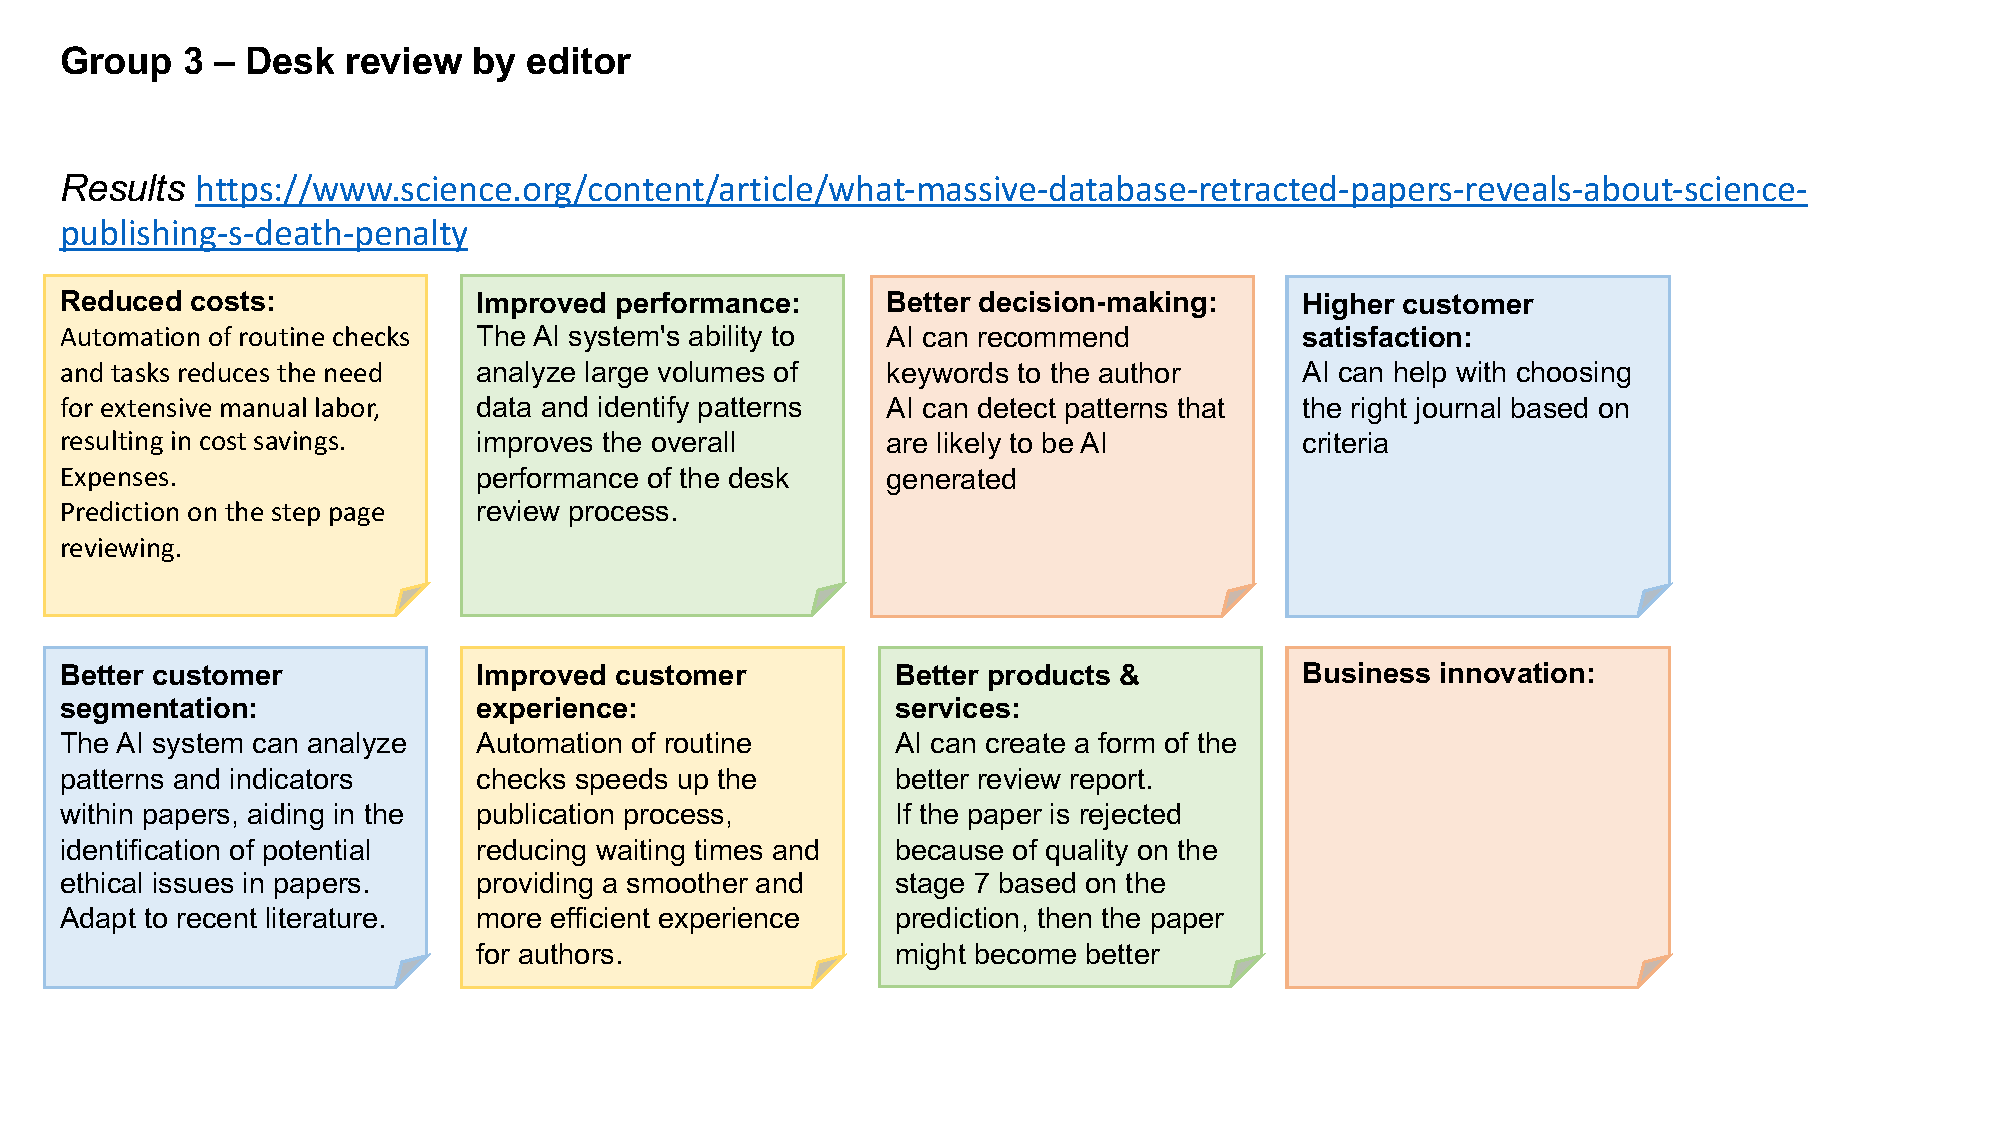
\includegraphics[width=\textwidth]{figures/results_3.pdf}
\end{figure}


\newpage
\subsection{Scenario 4: Finding Reviewers}

\subsubsection*{Scenario}

Once a manuscript passes desk review, the editors will send it to peer-review. To effectively peer-review a
manuscript, the editor will need to find subject experts that have previous experience with the type of research
reported in the manuscript. A hybrid, adaptive AI system could be employed to recommend suitable reviewers. The
editor may have additional rules for the selection of candidate reviewers (i.e., rules engineering or symbolic AI).
How could a hybrid AI combine sub-symbolic (e.g., word embeddings in vector space) and symbolic approaches (rules),
and how does such a system need to adapt? Hints: think of ca. November 2019 and early 2020 when the COVID pandemic
hit. Think of someone retiring. Think of a user that rejects certain recommendations. How would such a system help
the company to gain a competitive advantage?

\subsubsection*{Results}

The results for this scenario are shown in Figure~\ref{fig:appendix:fig4}.

\begin{figure}[h!]
    \centering
    \caption{Scenario 4: Finding Reviewers}
    \label{fig:appendix:fig4}
    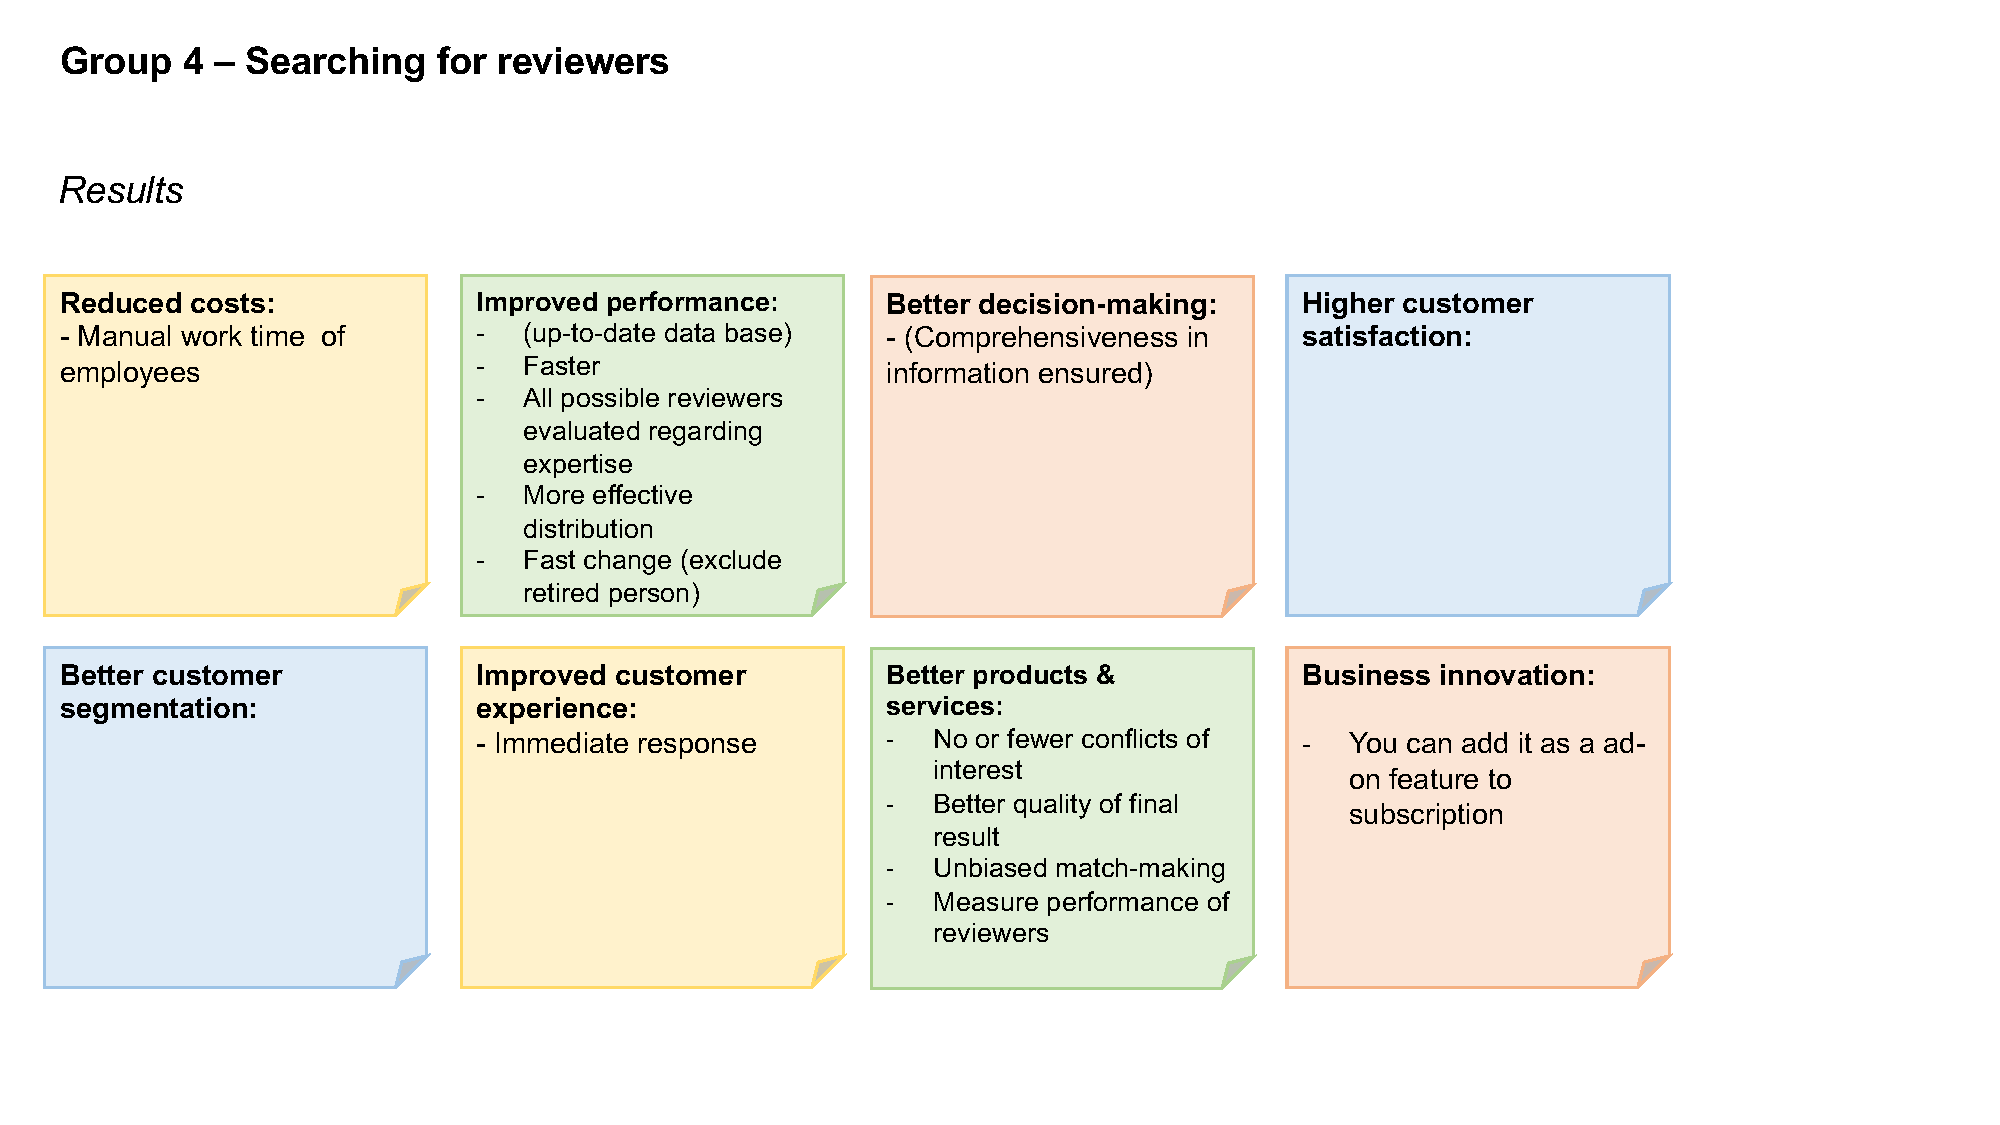
\includegraphics[width=\textwidth]{figures/results_4.pdf}
\end{figure}








    

